% ICIDS 2026 Late-Breaking Works — anonymised submission
% Build:  tectonic main.tex   (fetches packages on first run; bibtex handled automatically)
% Word budget: 2000–3000 words excluding references (LBW track).
%
% Anonymisation switch (2026-09-15): system name replaced by placeholder for double-blind review.
% To submit under a placeholder instead, change the two \newcommand lines below, e.g.
%   \newcommand{\sys}{Project M}  \newcommand{\sysshort}{PM}
\documentclass[runningheads]{llncs}

\usepackage[T1]{fontenc}
\usepackage{graphicx}
\usepackage{booktabs}
\usepackage{amsmath}
\usepackage{array}

\newcommand{\sys}{Project M}
\newcommand{\sysshort}{PM}

\begin{document}

\title{Measuring Emotional Trajectory Divergence in Interactive Narrative:\\ Alignment and Contamination Metrics in \emph{\sys}}
\titlerunning{Measuring Emotional Trajectory Divergence in Interactive Narrative}

% camera-ready (채택 후에만 교체): \author{Dohhan Park\orcidID{0009-0002-1385-8260}} \authorrunning{D. Park} \institute{Independent Researcher, Seoul, Republic of Korea}
\author{Anonymous Author(s)}
\authorrunning{Anonymous}
\institute{Anonymous Institution}

\maketitle

\begin{abstract}
Interactive narratives promise every participant a different experience, yet that difference is almost always described as a difference in plot branches. We present \emph{\sys} (\sysshort), a working browser-based interactive narrative in which the participant's emotional trajectory, not a branching graph, determines which scenes become accessible each turn, together with two computable metrics for how that trajectory departs from the author's: a real-time \emph{alignment} score that compares the shape of emotional change independently of its level, and a two-axis \emph{contamination} vector that separates directional \emph{drift} from single-point \emph{fixation}. Trajectories that reach \emph{contact} with the author's are converted automatically into interpretive fragments for later participants. A 193-play persona simulation shows that the alignment metric discriminates personality profiles ($r = 0.55$--$0.63$) while exposing a ceiling bias in LLM-simulated readers; a three-participant human pilot (21 scene-plays) exhibits the low tail the simulation lacked and shows three readers diverging onto distinct scene sequences without any authored branch.

\keywords{Interactive narrative \and Emotional trajectory \and Affective computing \and Reader modelling \and Drama management}
\end{abstract}

% ─────────────────────────────────────────────────────────────
\section{Introduction}

The central promise of interactive narrative is that each participant has a different experience. Since Murray's \emph{Hamlet on the Holodeck}~\cite{murray1997}, the tools that deliver this promise---Twine, Ink, articy:draft, and research systems such as StoryAssembler~\cite{garbe2019} and Versu~\cite{evans2014}---have concentrated on the diversity of \emph{paths} through a branching plot. The \emph{emotional trajectory} a participant traces while passing through the work is not tracked as a first-class quantity.

Affective computing does not close this gap. Quantitative models of emotion are well established~\cite{russell1977,watson1988,warriner2013}, and the Temporal Interpersonal Emotion Systems (TIES) framework~\cite{butler2011,butler2017}, with its computational form CompTIES~\cite{butlercomp2017}, shows that the dynamic pattern of emotion predicts experiential quality. These are, however, post-hoc tools fitted to observed data; none compares trajectories in real time inside a narrative. Reagan et al.~\cite{reagan2016} showed that stories' emotional arcs collapse onto six shapes, but that is a comparison \emph{between works}, not between two people who experienced the \emph{same} work.

This late-breaking paper reports a working system and its metrics, built to ask three questions.
\begin{description}
  \item[R1.] Can an interactive narrative operate on the participant's emotional trajectory alone, with no plot branching?
  \item[R2.] Can the way a participant's trajectory departs from the author's be measured quantitatively and separated into distinct modes?
  \item[R3.] Can a trajectory that reaches a particular affective relation to the author's be converted automatically into an interpretive fragment for the next participant?
\end{description}

We contribute (1)~\sysshort, an interactive narrative system whose scene access is a function of emotional distance and in which transition patterns move the \emph{centre} of the accessible region rather than its radius; (2)~two metrics, \emph{trajectory alignment} and a \emph{contamination} vector with separable drift and fixation axes; and (3)~a pilot validation: a 193-play persona simulation that shows internal discriminability and measures the instrument's own ceiling bias, and a 21-scene-play human pilot that exhibits the low tail the simulation lacked. We claim no theory of memory. We claim a measuring device, and an environment in which the measured quantity is what gets rendered.

% ─────────────────────────────────────────────────────────────
\section{Related Work}

\paragraph{Drama management without a branching graph.}
The idea that a system rather than an authored graph chooses the next narrative unit is well established. Fa\c{c}ade~\cite{mateas2005} selects beats toward an authored tension curve; search-based drama management~\cite{weyhrauch1997} formalised this; PaSSAGE~\cite{thue2007} added player modelling; and the lineage is now called experience management~\cite{riedl2013}. \sysshort{} shares the absence of a branching graph but departs on three points. First, the objective runs the other way: a drama manager optimises toward a target trajectory and treats deviation as error, whereas \sysshort{} steers toward nothing---the author's trajectory is a \emph{baseline for measurement}, and divergence from it is the rendered content. Second, there is no latent player model; the engine computes a geometric relation between two sequences each turn and neither classifies nor recommends. Third, the selection space is a neighbourhood on an affective manifold whose centre shifts with the transition pattern. The most verifiable difference is at the schema level: even beat-based managers keep pre- and post-conditions that leave a partial plot graph, while \sysshort's choice records carry no next-scene column at all (Sect.~\ref{sec:data}).

\paragraph{Comparing emotional trajectories.}
Emotional convergence between people has been studied longitudinally~\cite{anderson2003}, and CompTIES~\cite{butlercomp2017} fits coupled-oscillator models to rating-dial recordings after the fact. \sysshort's alignment metric (Sect.~\ref{sec:alignment}) transplants the TIES principle---that the shape of change predicts similarity independently of its level---into a real-time engine inside an interactive narrative.

\paragraph{Reader traces passed forward.}
Mechanisms for leaving one reader's trace to the next include the anonymous messages of \emph{Dark Souls}~\cite{fromsoftware2011}, anchored to spatial position; web annotation layers such as Hypothesis; and Genius-style commentary ranked by popularity. \sysshort's trajectory bridges (Sect.~\ref{sec:bridges}) are closest to the first but anchor to an \emph{emotional} axis, and they refuse popularity ranking: exposure is conditioned on alignment with the current participant's state.

\paragraph{Memory as reconstruction.}
That recall reconstructs rather than retrieves~\cite{bartlett1932,loftus1974,nader2000,hirst2012} is the background against which \sysshort{} was designed. This paper makes no cognitive claim; it isolates one facet---divergence of emotional trajectory---and makes it measurable inside a narrative.

% ─────────────────────────────────────────────────────────────
\section{\sys}

\sysshort{} is a browser-based interactive narrative with two modes. In \emph{Record}, an author structures a personal memory into scenes through an AI-mediated conversation. In \emph{Play}, a participant traverses another person's memory scene by scene, supplying an emotional response at every turn as a short continuation of the text or a choice. A third view, \emph{strata}, lays every scene out as a three-dimensional terrain positioned by a valence--arousal projection of its emotion distribution, navigated in first person with spatialised audio; contour depth accumulates from past plays, so the terrain records collective traversal. The runtime is deterministic and covered by regression tests.

\subsection{Data Model}
\label{sec:data}

\begin{table}[t]
\caption{Core entities of \sysshort.}
\label{tab:data}
\centering
\footnotesize
\begin{tabular}{@{}l >{\raggedright\arraybackslash}p{4.9cm} >{\raggedright\arraybackslash}p{4.0cm}@{}}
\toprule
\textbf{Entity} & \textbf{Key fields} & \textbf{Meaning} \\
\midrule
memory & id, title, meta & one authored memory \\
scene & memory\_id, scene\_order, text, original\_emotion, echo\_words, text\_stage\_1/2/3 & one scene; \texttt{original\_emotion} is a distribution over emotion labels \\
choice & scene\_id, emotion, intensity & an option inside a scene; records affective colour only; \textbf{no next\_scene\_id} \\
play & memory\_id, trajectory\_data & one participant's traversal \\
trajectory\_bridge & memory\_id, scene\_id, source\_run\_id, entry\_emotion, key\_passed\_scenes & automatic record of a contact run \\
\bottomrule
\end{tabular}
\end{table}

Table~\ref{tab:data} lists the core entities. The absence of a \texttt{next\_scene\_id} column is deliberate: a choice changes the participant's emotional state, and the next scene is a function of that state. All emotion comparisons are taken in a \emph{memory-local frame}, the set of labels the author actually used in that memory (a 17-label default vocabulary serves as fallback), so that a memory written largely in \emph{longing} is measured on that axis rather than on a fixed global basis.

\subsection{Scene Access by Emotional Trajectory}
\label{sec:access}

Each turn, given the participant's current emotion distribution $u_t$ and each scene's original distribution $o_s$, the system computes
\begin{equation}
d(s,t) = 1 - \cos(u_t, o_s),
\end{equation}
takes the scenes with $d \le \tau$ as candidates, weights them by recency of visit, and presents the top $k$ as accessible pins. Crucially, the transition pattern reported by the engine (Sect.~\ref{sec:alignment}) shifts the \emph{centre} of this region rather than its radius: \emph{echo\_follow} biases the centre toward the original, \emph{contradiction} toward the opposite of the participant's current state, \emph{avoidance} toward neutral ground. If patterns changed only the radius, the engine would degrade into a lookup table. The consequence is that two participants of the same work can see entirely different scene sequences; this is the concrete form of ``difference'' that we measure. The participant sees only a fogged local view of nearby accessible scenes; the author's tooling sees the whole map.

\subsection{Contact and Trajectory Bridges}
\label{sec:bridges}

We call \emph{contact} the rare event in which a participant's trajectory overlaps the author's beyond a threshold. Contact is neither an ending nor a reward; it is shown at most once per run. When it occurs, the run is converted automatically into a \emph{trajectory bridge}: the emotion state at entry, the key scenes passed, and the sentence the participant left last. Bridges are exposed to later participants in the strata view and in scene rendering, anonymously, and conditioned on alignment with the later participant's state rather than on popularity. A bridge is thus one participant's memory-within-a-memory; it coexists with the author's own static interpretive fragments. Figure~\ref{fig:pipeline} summarises the runtime loop.

\begin{figure}[t]
\centering
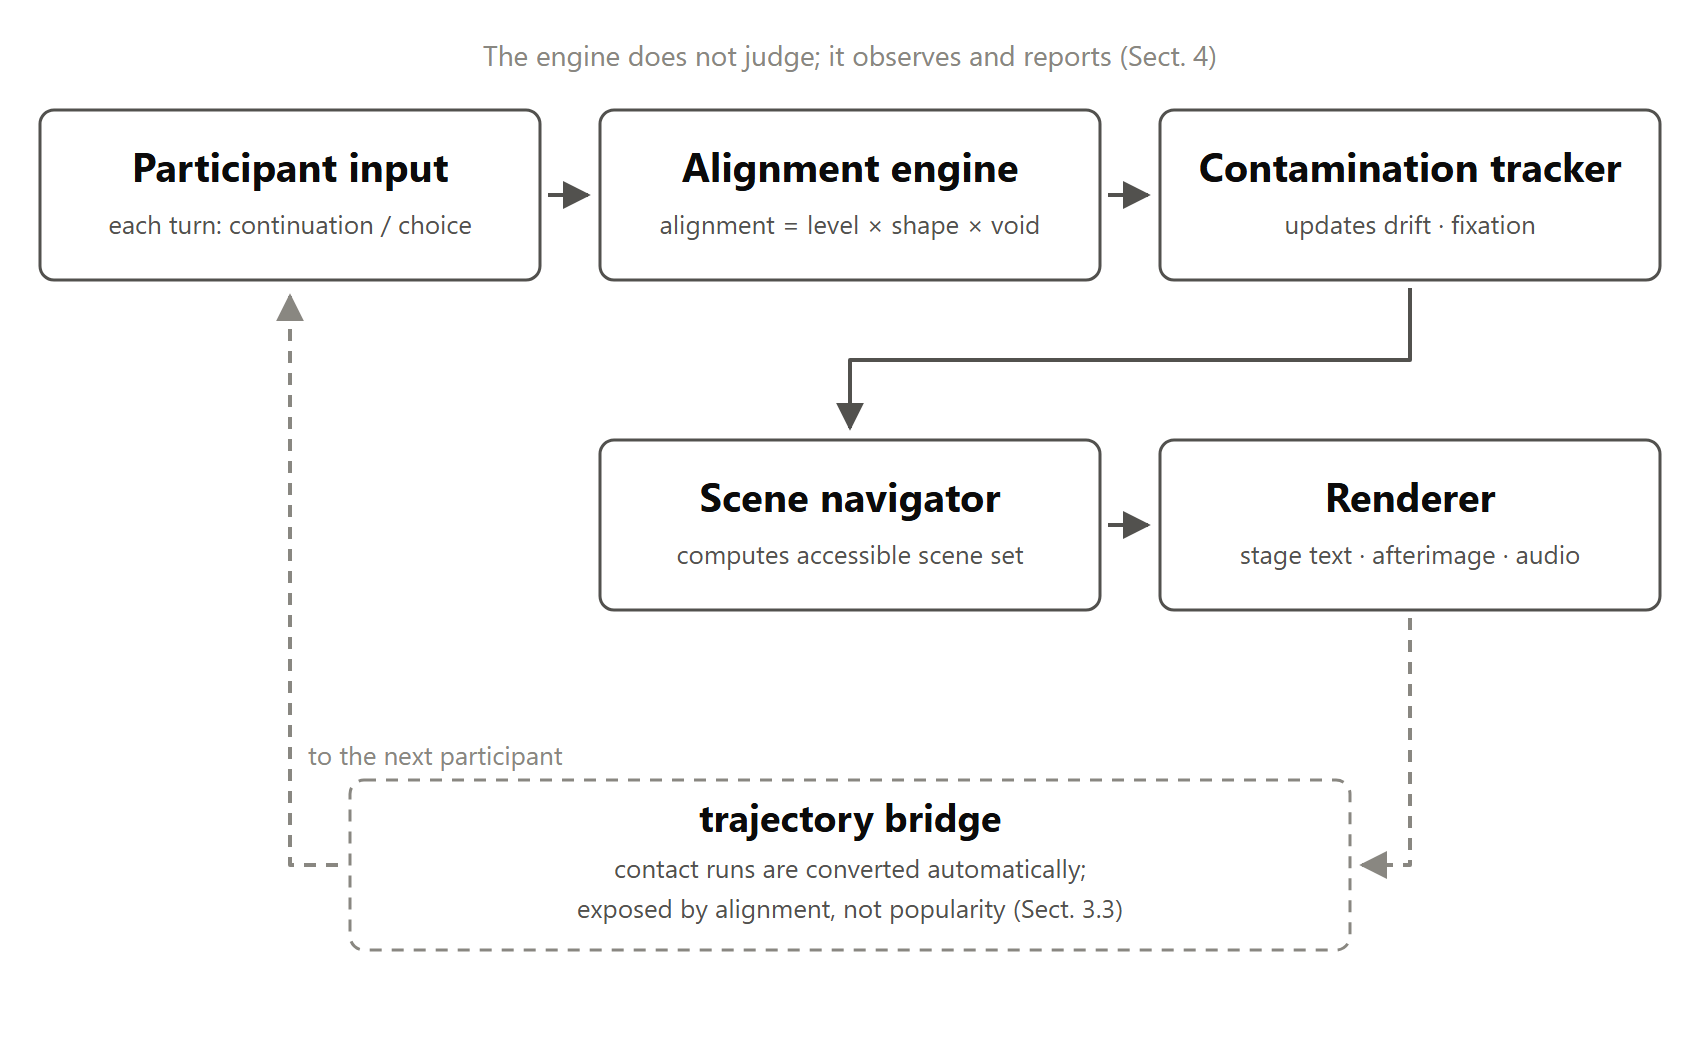
\includegraphics[width=\textwidth]{figures/fig1_pipeline_en.png}
\caption{Runtime loop. Each turn the participant's input passes through alignment (Sect.~\ref{sec:alignment}), contamination (Sect.~\ref{sec:contamination}), and accessible-scene computation (Sect.~\ref{sec:access}) before rendering. A contact run is converted into a trajectory bridge and exposed to later participants.}
\label{fig:pipeline}
\end{figure}

% ─────────────────────────────────────────────────────────────
\section{Metrics}

\subsection{Trajectory Alignment}
\label{sec:alignment}

The alignment engine scores the similarity between the participant's emotion sequence and the author's original sequence, every turn, as the product of three factors:
\begin{equation}
\text{alignment} = \operatorname{clamp}_{[0,1]}\big(\text{level} \times \text{shape} \times \text{void\_mod}\big).
\end{equation}
\emph{Level} is the mean, over visited scenes, of the per-scene cosine similarity between participant and original distributions. \emph{Shape} compares the trajectories of \emph{change}: with $\Delta u$ and $\Delta o$ the sequences of successive differences,
\begin{equation}
\text{shape} = \max\!\big(0,\ \cos(\operatorname{flatten}\Delta u,\ \operatorname{flatten}\Delta o)\big)
\end{equation}
once three or more scenes have been visited, and $1.0$ before that. The original sequence is re-ordered by the participant's visit order, because which scene one opens first is already an act of interpretation. \emph{void\_mod} is $0.7$ when the participant withheld an emotion where the author expressed one, and $1.0$ otherwise.

The factors are multiplied rather than added so that no factor can compensate for another: a level of zero yields zero alignment regardless of shape. That shape compares the \emph{direction} of change rather than its magnitude is the transplanted TIES principle; two people whose emotional levels differ can still share a high shape score. The engine is deterministic (snapshot-tested against golden fixtures), runs in time linear in the number of visited scenes, and is non-monotonic by design. Alongside the score it reports a bucket (HIGH/MID/LOW/FIXATED), a mismatch type, and a transition pattern from \{echo\_follow, bridge, contradiction, displacement, avoidance, fixation\}, which scene access consumes (Sect.~\ref{sec:access}). The engine does not judge; it observes and reports.

\subsection{Contamination: Drift and Fixation}
\label{sec:contamination}

The contamination vector measures two \emph{separate} modes of departure, each as an exponentially smoothed axis in $[0,1]$ updated from the engine's per-turn output. \emph{Drift} is directional departure: its per-turn signal is
\begin{equation}
\text{drift}_t = 0.45\,(1-\text{level}) + 0.35\,(1-\text{shape}) + 0.20\,b_{\text{mismatch}},
\end{equation}
where $b_{\text{mismatch}} \in [0,1]$ weights the reported mismatch type (emotion mismatch $1.0$, attribution mismatch $0.7$, target displacement $0.6$). \emph{Fixation} is over-staying on one emotion or attribution:
\begin{equation}
\text{fix}_t = 0.55\,f_{\text{sim}} + 0.25\,b_{\text{align}} + 0.20\,b_{\text{pattern}},
\end{equation}
where $f_{\text{sim}}$ is the mean pairwise cosine among the last three participant states, $b_{\text{align}}$ rises linearly from alignment $0.55$ to $1.0$, and $b_{\text{pattern}}$ is $1.0$ for the \emph{fixation} pattern and $0.5$ for \emph{echo\_follow}. Each axis is updated as $\alpha\,\text{signal}_t + (1-\alpha)\,\text{axis}_{t-1}$. The dominant stage is declared \emph{hypercompletion} when fixation $\ge 0.65$ and exceeds drift, and \emph{biased inclination} when drift $\ge 0.35$. The full three-signal fixation specification (similarity, attribution repetition, exploration rate) is only partially implemented; the current runtime uses the similarity signal alone.

Two axes are needed because the same total departure can feel entirely different: drift-dominant play ``wanders off onto another road'', fixation-dominant play ``gets stuck on one point and repeats''. Rendering decisions---which biased stage of a scene's text is shown, when a character's monologue is triggered---reference the two axes independently.

\subsection{Declared Limits}
(1)~Scene emotion distributions come from author self-report, alone or with AI assistance; convergent validity against independent raters is unmeasured. (2)~Participant input is discrete text or choices, not a continuous physiological signal. (3)~There is no ground truth for a ``correct'' trajectory; the metrics measure similarity and mode of departure, not accuracy.

% ─────────────────────────────────────────────────────────────
\section{Evaluation}

\subsection{Persona Simulation}
\label{sec:sim}

Fifteen synthetic participants were driven by an LLM on top of Big Five backbones stratified from a public IPIP-NEO response corpus ($N = 307{,}313$)~\cite{goldberg1999,johnson2014}. On a single ten-scene memory they produced 193 plays (seed 42; two to four visits per persona). The measured quantity is the \emph{per-scene alignment score}, the level component of Sect.~\ref{sec:alignment}: the cosine similarity between the persona's emotion distribution and the scene's original distribution. The LLM's own self-reported alignment was also logged, as a comparison signal only.

\paragraph{Distribution.}
Per-scene alignment had mean $0.809$, SD $0.149$, range $0.254$--$0.986$. Mismatch was flagged on $97.4\%$ of scene-plays, with \emph{target\_displacement} dominant ($82.4\%$). Self-reported alignment collapsed onto three values ($71.0\%$ of cases), confirming that alignment must be computed from distributions rather than asked.

\paragraph{H1: personality discriminates alignment.}
Table~\ref{tab:corr} gives Pearson correlations between each Big Five trait and mean alignment across the 15 personas ($|r| \ge 0.51$ corresponds to $p < .05$). Openness, Agreeableness, and Extraversion predicted alignment; Conscientiousness and Neuroticism did not. Openness as the strongest predictor was not anticipated.

\begin{table}[t]
\caption{Correlation between Big Five trait and mean per-scene alignment ($n = 15$ personas).}
\label{tab:corr}
\centering
\begin{tabular}{@{}lll@{}}
\toprule
\textbf{Trait} & $r$ & \textbf{Reading} \\
\midrule
Openness & \textbf{0.634} & significant; strongest, unanticipated \\
Agreeableness & \textbf{0.590} & significant; as predicted \\
Extraversion & \textbf{0.549} & significant \\
Conscientiousness & 0.192 & not significant \\
Neuroticism & 0.131 & not significant \\
\bottomrule
\end{tabular}
\end{table}

\paragraph{H2: extreme personas form the tails.}
The cynical persona (low Agreeableness, low Conscientiousness) ranked last ($0.638$) and produced the low tail. The extreme-optimist persona, designed to fail at empathising with the memory's shadow, ranked seventh ($0.840$): negative extremes are simulated, but \emph{empathic failure is not}. This asymmetry is a property of the instrument.

\paragraph{H3: ceiling bias.}
All fifteen personas averaged above $0.64$, and no scene-play fell below $0.25$. LLM-simulated readers over-resonate: sampling personality from a real distribution does not remove the upward bias introduced at the response-generation step. The instrument is therefore valid for \emph{relative} comparison but ceiling-biased in \emph{absolute} distribution. We read this as a measured boundary rather than a failure.

\subsection{Human Pilot}
\label{sec:pilot}

In a closed alpha (August 2026) three participants completed one run each of a second authored memory, yielding 21 scene-plays. The formula is identical to Sect.~\ref{sec:sim}; values stored by the live system were recomputed offline and matched in all 21 cases. Human emotion distributions are extracted by an LLM from the participant's free-text continuation, whereas persona distributions are produced directly by the role-playing LLM; both pass through an LLM but from different input modalities.

\begin{table}[t]
\caption{Per-scene alignment, human pilot versus persona simulation (same formula).}
\label{tab:pilot}
\centering
\begin{tabular}{@{}l@{\hspace{2em}}l@{\hspace{2em}}l@{}}
\toprule
 & \textbf{Human pilot} ($n=21$) & \textbf{Persona sim.} ($n=193$) \\
\midrule
Mean & 0.517 & 0.809 \\
SD & 0.211 & 0.149 \\
Range & 0.114--0.781 & 0.254--0.986 \\
Share $< 0.42$ & 28.6\% & 3.1\% \\
Share $< 0.25$ & \textbf{14.3\%} & \textbf{0.0\%} \\
\bottomrule
\end{tabular}
\end{table}

\begin{figure}[t]
\centering
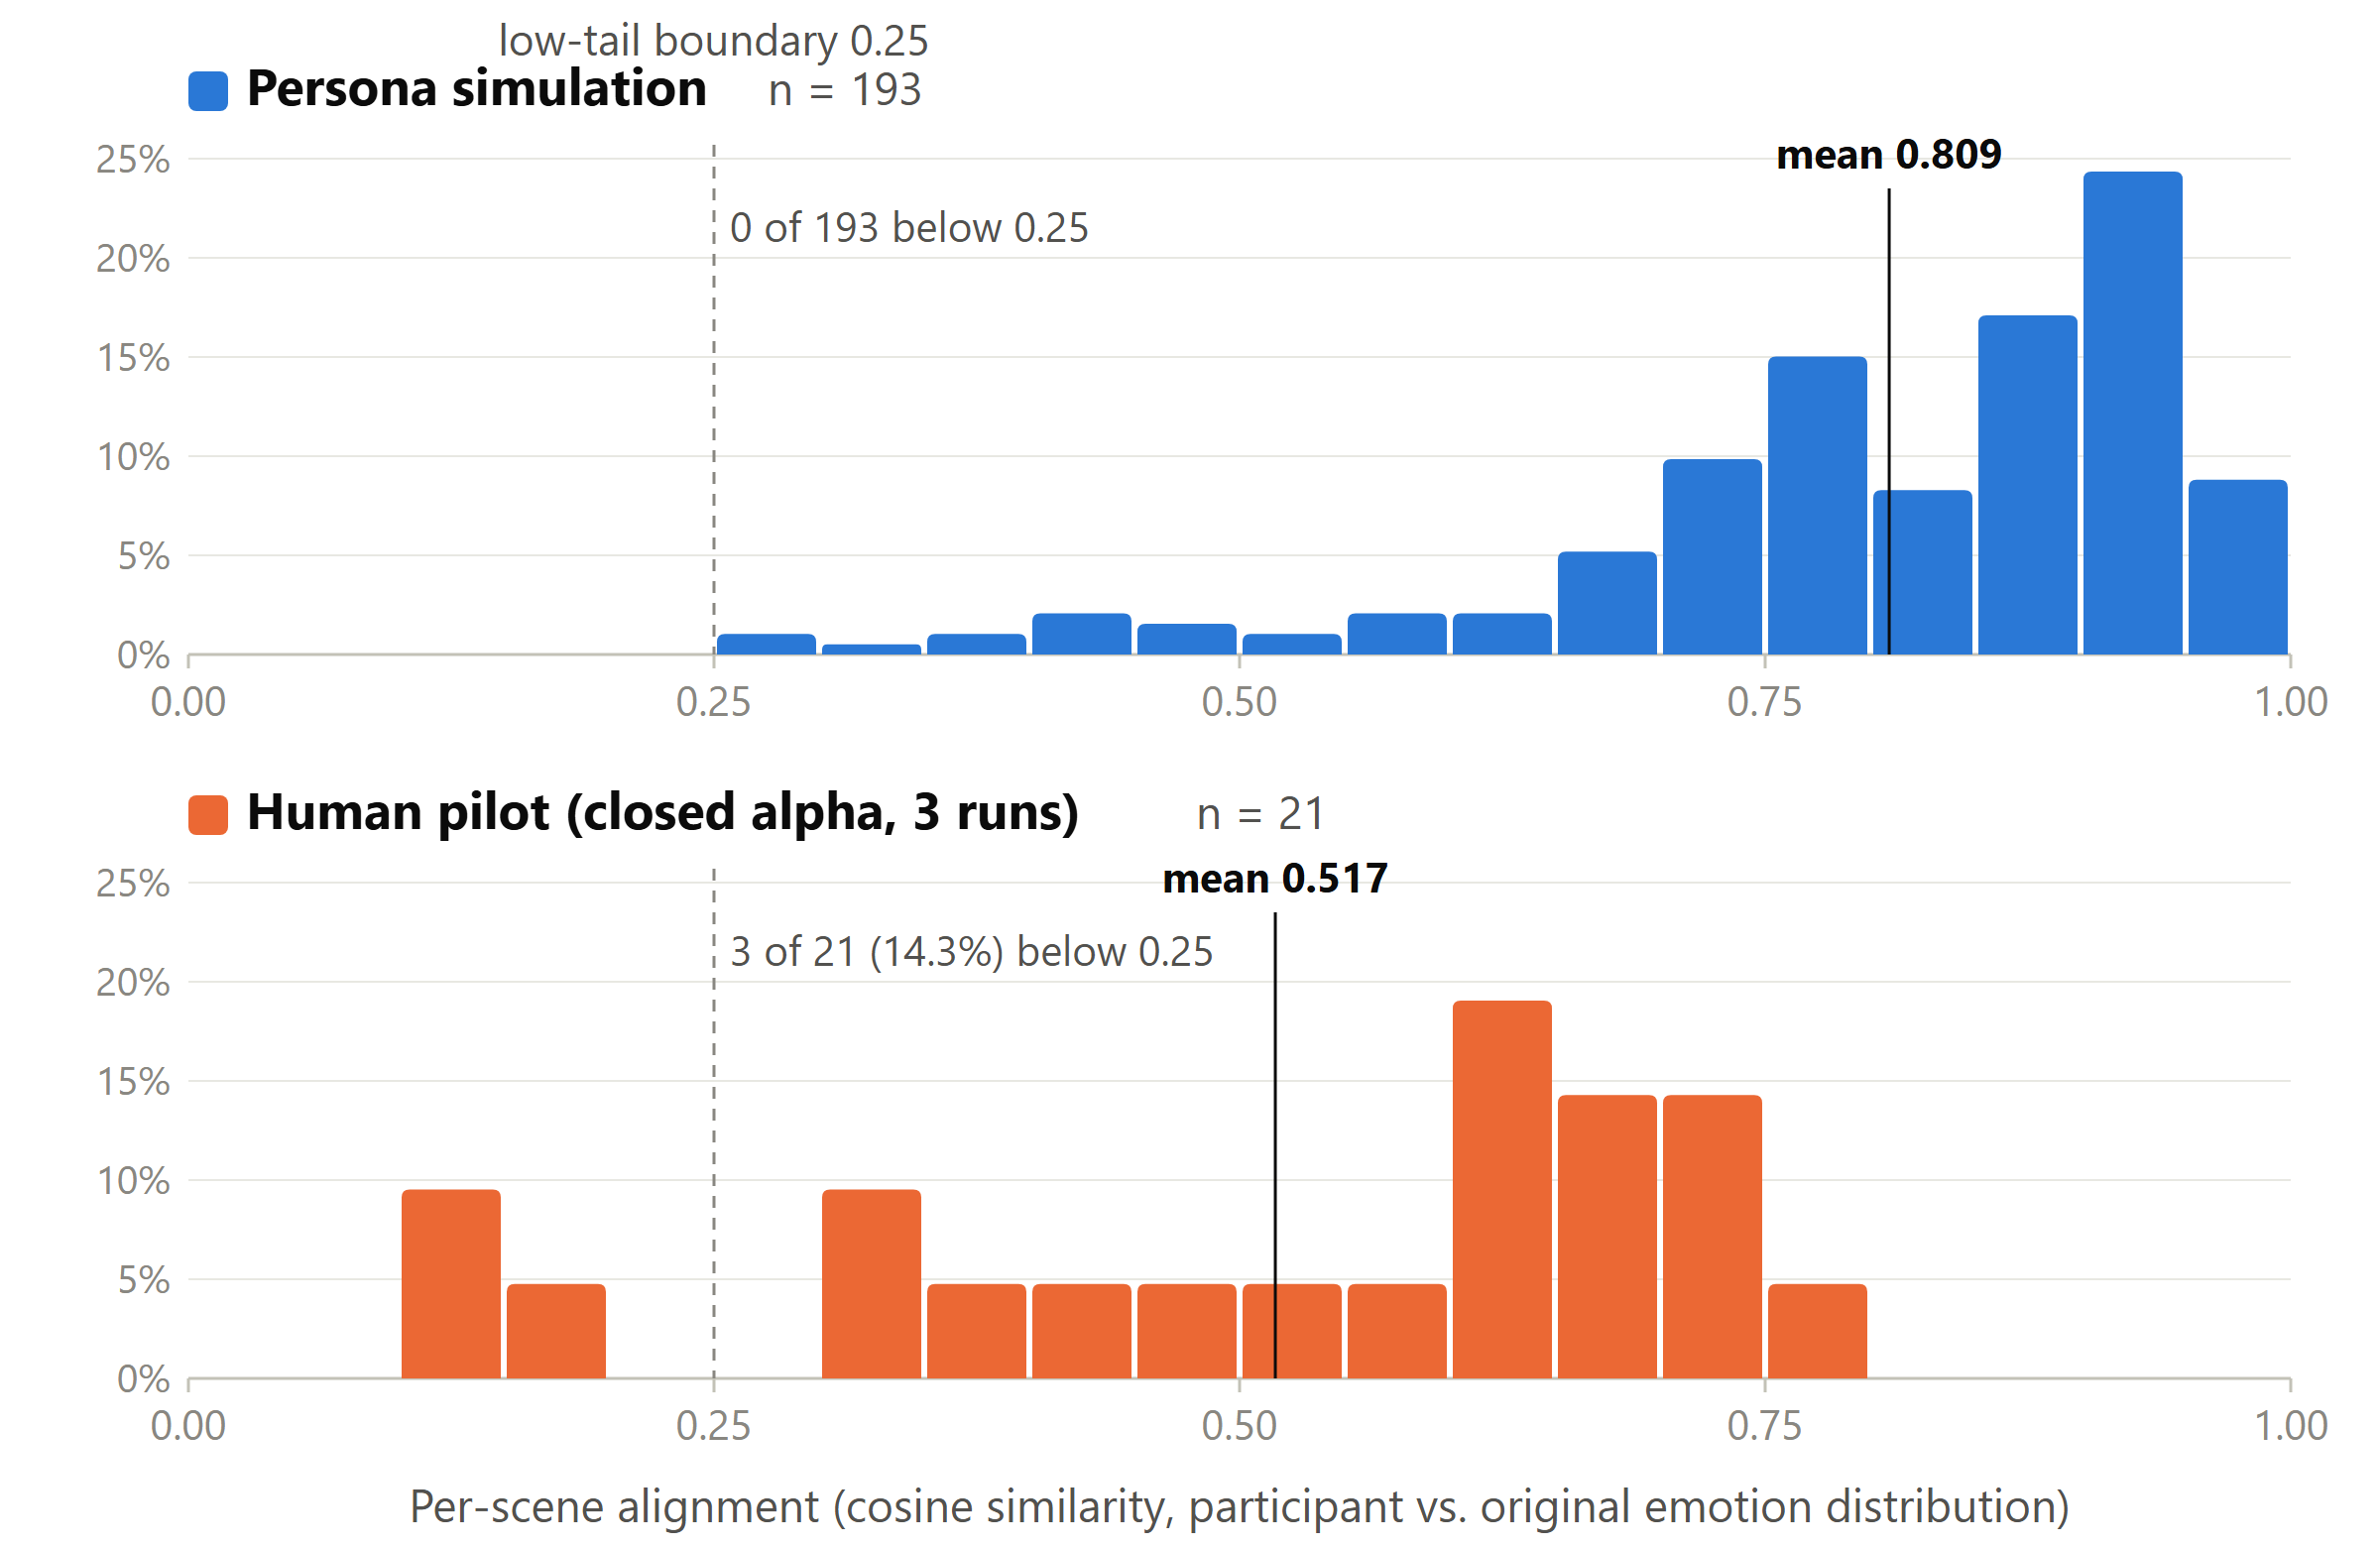
\includegraphics[width=0.92\textwidth]{figures/fig2_dist_en.png}
\caption{Per-scene alignment distributions under the same formula. Top: persona simulation, no case below $0.25$. Bottom: human pilot, $14.3\%$ below $0.25$. The low tail the simulation could not reproduce is present in human data.}
\label{fig:dist}
\end{figure}

Three things are observed (Table~\ref{tab:pilot}, Fig.~\ref{fig:dist}). \emph{First, the low tail is real.} Sect.~\ref{sec:sim} reported the absence of a tail below $0.25$ as an assumption about human readers; $14.3\%$ of human scene-plays fell below it (minimum $0.114$), against none of 193 simulated. This is the first human signal consistent with the ceiling-bias boundary. \emph{Second, dispersion is wider.} The human SD ($0.211$) is $1.4\times$ the simulation's, and the three run means ($0.633$, $0.522$, $0.456$) sit at distinct heights. \emph{Third, path divergence was observed in human trajectories} (Fig.~\ref{fig:paths}). The three scene sequences share their first three visits and diverge at the fourth. We read the shared prefix as a consequence of design rather than a defect: the shape factor activates only from the third scene, so trajectory-based access has a warm-up interval. Whether the prefix length coincides with shape activation is testable once more runs accumulate.

\begin{figure}[t]
\centering
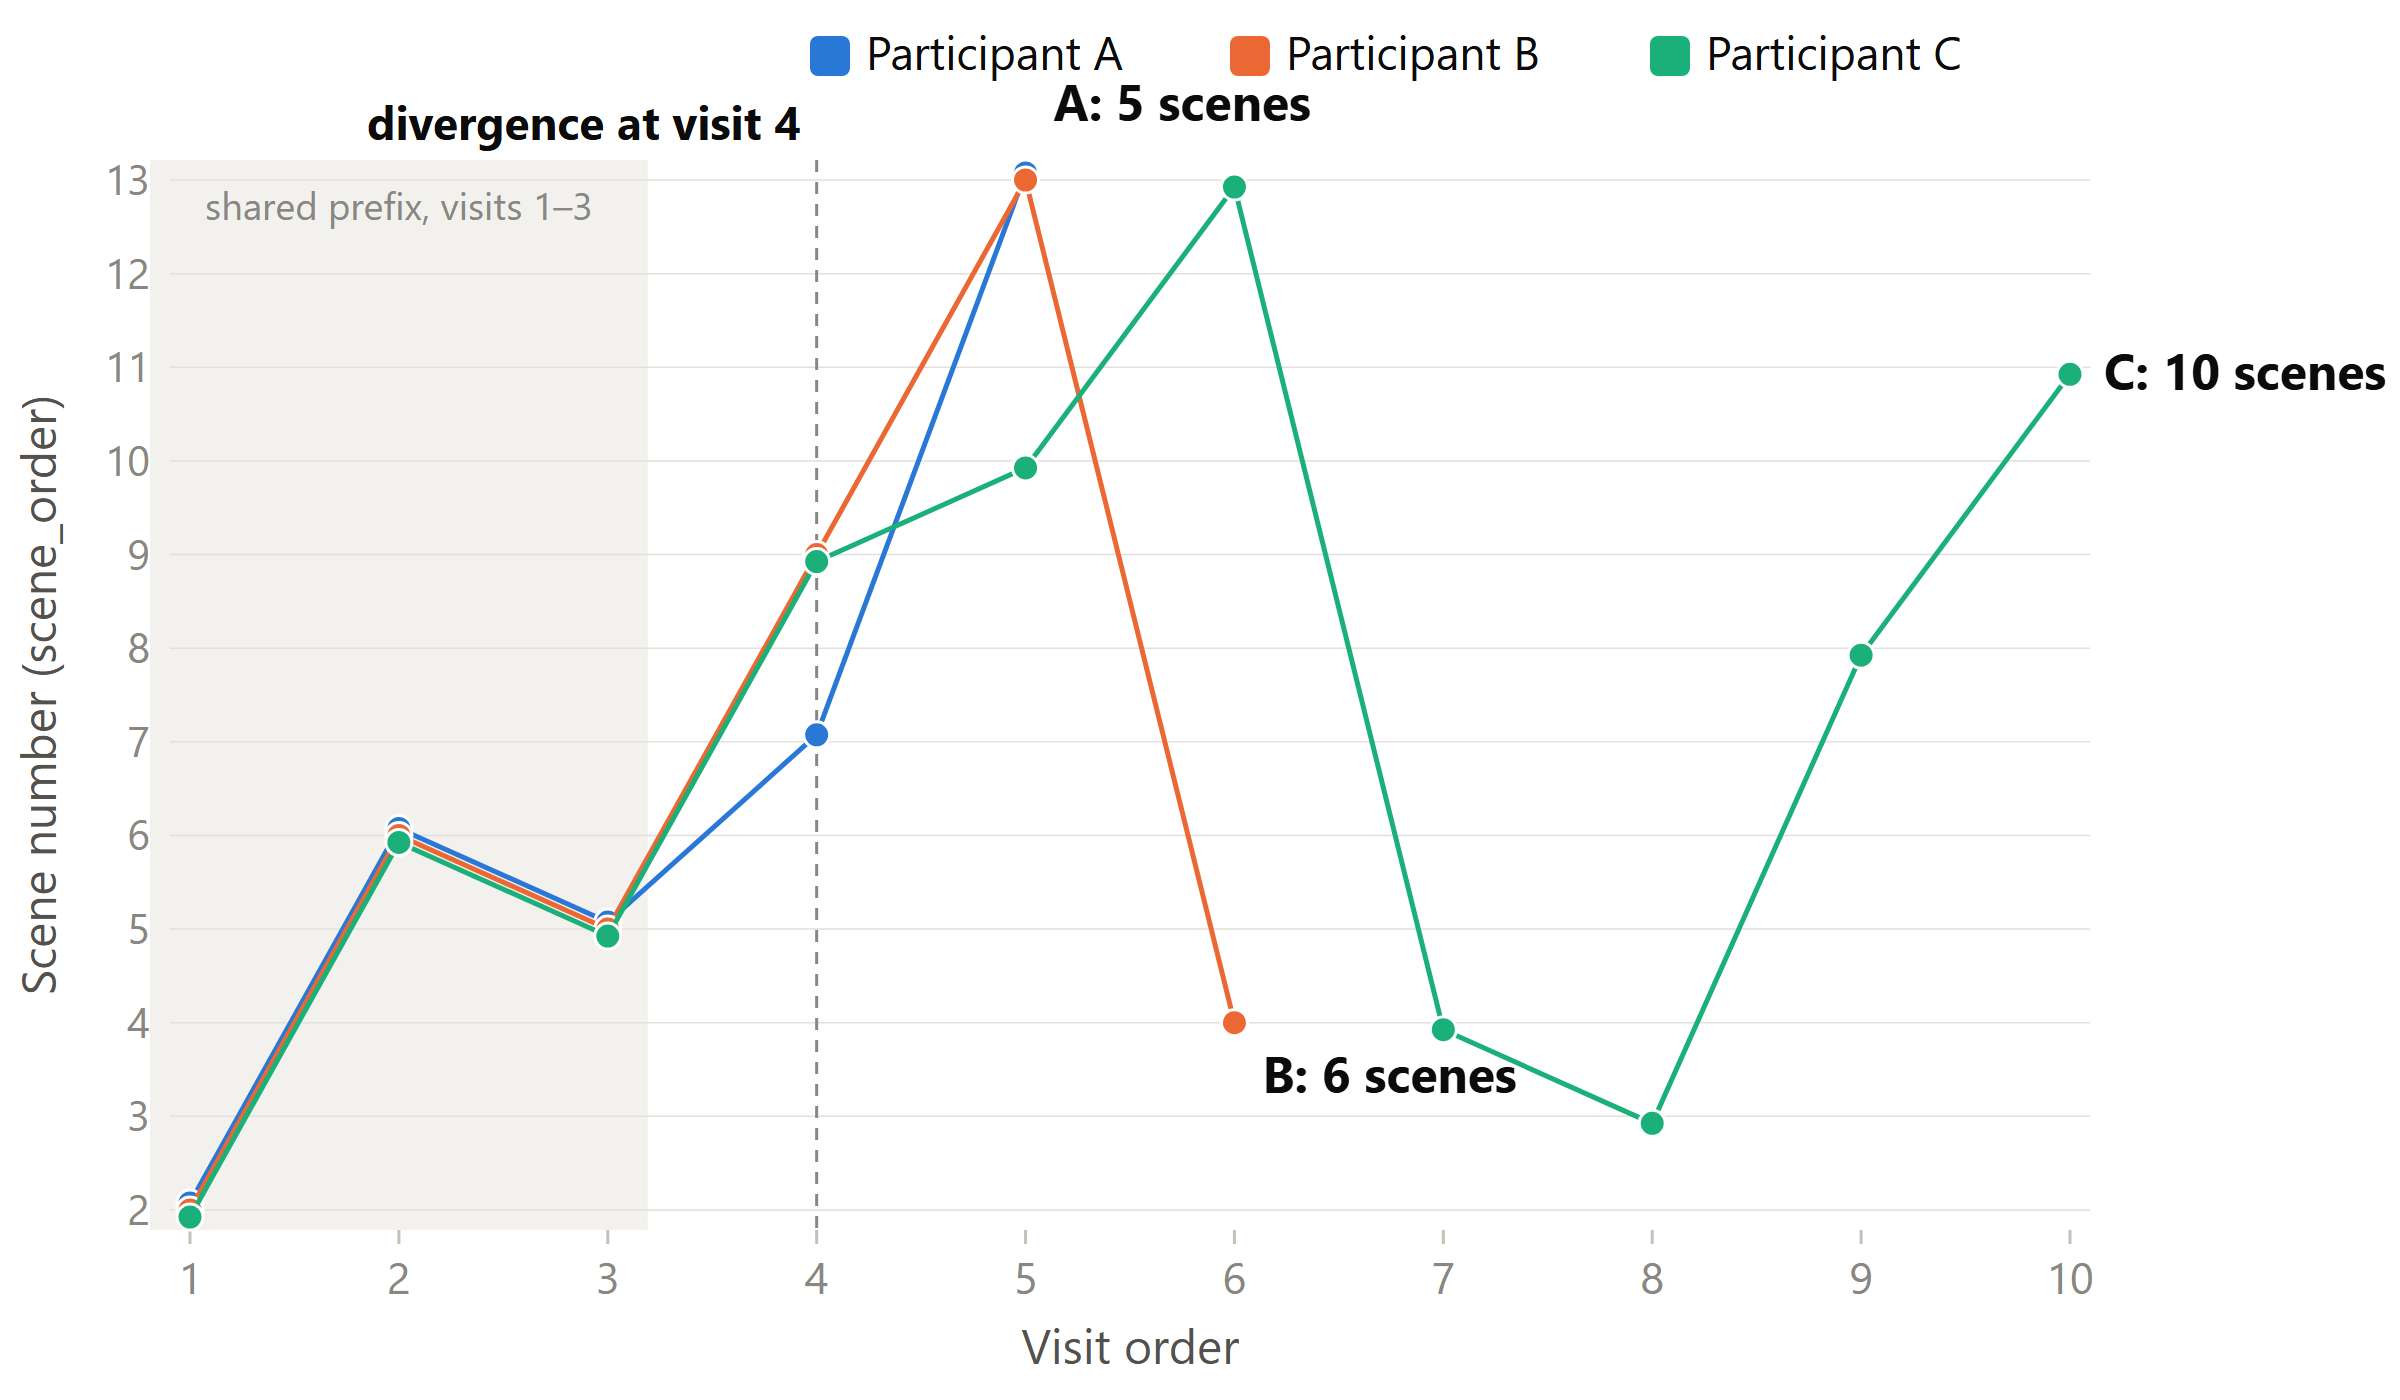
\includegraphics[width=0.9\textwidth]{figures/fig3_paths_en.png}
\caption{Scene sequences of the three pilot participants. The first three visits coincide; divergence begins at the fourth visit, with no authored branch in the data. Overlapping segments are offset vertically by a few pixels.}
\label{fig:paths}
\end{figure}

\paragraph{What this does not claim.}
The pilot was collected on a \emph{different} memory from the simulation, so part of the $0.292$ mean gap may be a work effect; until same-work human data exist the comparison is valid only for distribution shape (tail and dispersion). Mismatch types were excluded because the two populations used different classifiers. $n = 3$ is a convenience sample without ethics-board review; it is a directional signal, not a statistical claim.

% ─────────────────────────────────────────────────────────────
\section{Limitations and Future Work}

Scene emotion distributions rest on author self-report and need cross-author or independent-rater validation. The fixation composite is partially implemented; results labelled FIXATED currently reflect the similarity signal alone. LLM personas import the LLM's affective biases, which multi-model comparison or human calibration must bound. The contact threshold is heuristic and has no sensitivity analysis. Finally, some authored turning points are hard to induce by emotional distance alone; an author-side ``port'' mechanism is being designed within a budget of roughly 15\% of scenes so that the engine is not reduced to decoration.

Next steps are (i)~a human study ($N = 30$--$50$) on the same memory as the simulation, testing the two pilot contrasts---the low tail and the $1.4\times$ dispersion---while removing the work confound; (ii)~tracking alignment, drift, and fixation \emph{after} a participant is exposed to a trajectory bridge, to measure whether bridges alter later trajectories; and (iii)~cross-work replication, to separate whether the $82.4\%$ dominance of \emph{target\_displacement} is driven by the memory's topic or by classifier bias.

Emotional input is sensitive data. Authors consent at recording time to their fragments being exposed to later participants; a filter removes personally identifying content from exposed fragments; trigger-word handling escalates over turns rather than blocking outright; and bridges are traceable to a run identifier internally but never rendered with any author identity.

% ─────────────────────────────────────────────────────────────
\section{Conclusion}

Interactive narrative has long promised a different experience to every participant; few tools say what that difference \emph{is} in emotional terms. We presented a working system in which the participant's emotional trajectory, not a branching graph, determines scene access; a real-time alignment metric that compares the shape of emotional change; a contamination vector that separates drift from fixation; and a mechanism that turns contact runs into interpretive fragments for later participants. A 193-play simulation established internal discriminability and the instrument's ceiling bias; a 21-scene-play human pilot showed the tail and dispersion the simulation lacked, and three readers walking different scene sequences with no authored branch. What we offer is not a theory but a measuring device, and an environment in which what it measures is what is rendered.

% ─────────────────────────────────────────────────────────────
\bibliographystyle{splncs04}
\bibliography{refs}

\end{document}
